% !TEX root = main.tex

\section{网络层}
\subsection{IP数据报}
\subsubsection{数据传输技术}
\begin{itemize}
\item 电路交换(circuit switching):实际接通一条物理线路,时分多路复用,电话;频分多路复用,电视;一直占用,不管有无数据交互
\item \textemph{包交换/分组交换}\footnote{所以IP数据报也被称为IP分组(packet)}(packet switching):统计多路复用,按需分配;可能引起网络拥塞,适合发送突发数据
\begin{itemize}
	\item 虚电路:\textemph{需建立连接}才可以传输数据(仿照电话系统,恒变位速率ATM,因特网之前),好处在于保留带宽
	\begin{itemize}
	    \item 交换式(要交换才建立连接):建立虚电路(VC)表,虚电路标识符(VCI),类似于电话
	    \item 永久式(建立后一直保持):由管理员维护
	\end{itemize}
	\item 数据报(datagram):不需建立连接,因特网,\textemph{不预留带宽}
\end{itemize}
\begin{figure}[H]
	\centering
	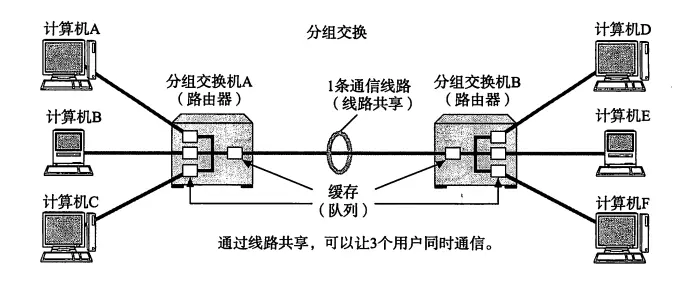
\includegraphics[width=0.6\linewidth]{fig/ip-packet.png}
\end{figure}
\end{itemize}

\begin{example}
	下图存在3条虚电路(红绿蓝) ,它们都是从A或者B出发的虚电路,请填写它们的虚电路表。
	接口编号用黑色字表示。 VCI - Virtual Circuits Identifier
	\begin{figure}[H]
		\centering
		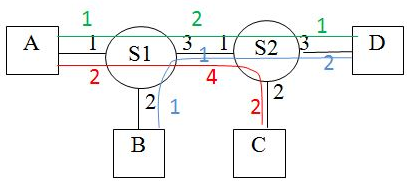
\includegraphics[width=0.4\linewidth]{fig/virtual_circuit.png}
	\end{figure}
\end{example}
\begin{analysis}
交换机S1的虚电路表
\begin{center}
\begin{tabular}{ccccc}\hline
 & 输入接口 & 输入VCI & 输出接口 & 输出VCI\\\hline
红 & 1 & 2 & 3 & 4\\
绿 & 1 & 1 & 3 & 2\\
蓝 & 2 & 1 & 3 & 1\\\hline
\end{tabular}
\end{center}
交换机S2的虚电路表
\begin{center}
\begin{tabular}{ccccc}\hline
 & 输入接口 & 输入VCI & 输出接口 & 输出VCI\\\hline
红 & 1 & 4 & 2 & 2\\
绿 & 1 & 2 & 3 & 1\\
蓝 & 1 & 1 & 3 & 2\\\hline
\end{tabular}
\end{center}
\end{analysis}

一般网络的服务模型:Aynchronous Transfer Mode, ATM
\begin{center}
\begin{tabular}{|c|c|c|c|c|c|c|}\hline
网络结构 & 服务模型 & 带宽 & 不丢包 & 有序 & 及时 & 拥塞反馈\\\hline
ATM & 恒定位速率 & 固定速率 & 是 & 是 & 是 & 无拥塞\\\hline
ATM & 可变位速率 & 确保速率 & 是 & 是 & 是 & 无拥塞\\\hline
ATM & 可用位速率 & 最小保证 & 否 & 是 & 否 & 是\\\hline
ATM & 未指定位速率 & 无 & 否 & 是 & 否 & 否\\\hline
因特网 & 尽力服务 & 无 & 否 & 否 & 否 & 否\\\hline
\end{tabular}
\end{center}

\myhline
IP协议是\textemph{因特网的网络层协议}
\begin{itemize}
\item 可路由的(routable):全局地址,按层分配
\item 尽力服务(best effort):\textemph{无连接无确认}的\textemph{数据报}服务,不可靠的
\item IP协议可以运行在\textemph{任何物理网络}上,不仅仅是因特网
\end{itemize}
注意:IP协议不具有拥塞控制机制

\subsubsection{数据报格式}
\begin{figure}[H]
	\centering
	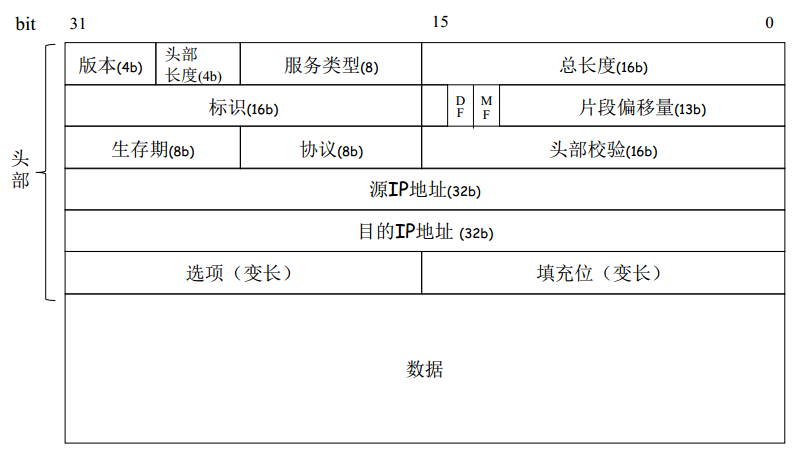
\includegraphics[width=0.7\linewidth]{fig/IP_datagram.png}
\end{figure}
\begin{itemize}
\item 版本:共两个版本,IPv4为4,IPv6为6
\item 头部长度:以\textemph{字(32b)}为单位
\item 服务类型(Type of Service, ToS):现在重新定义为\textemph{区分服务}
\item 总长度:整个数据报的长度,以\textemph{字节}为单位
\item 标识(identification)、标志(DF/Dont fragment、MF/More fragment)、偏移量:用于划分片段
\item 生存期(Time-to-live, TTL):
\begin{itemize}
	\item \underline{防止数据报长时间滞留在因特网上},实际限制为经过的路由器数目,即跳数(hop count),每经过一个路由器减1,超过则自动清除,防止兜圈,同时发送ICMP包告知源主机
	\item TTL初值默认设置为\textemph{网络直径的两倍},Windows默认64,Unix默认为255
	\item 长了就有捷径(cut-through),因此发展到现在因特网的直径依然在32左右,即TTL\underline{限制了因特网的直径}
\end{itemize}
\item 协议:\underline{TCP为6,UDP为17,ICMP为1,IGMP为2}
\item 头部选项:1B代码,1B总长度,nB数据
\begin{itemize}
	\item 4个字节一个字,头部最多$(2^4-1)*4=60$B,除去非选项部分$4*5=20$B,IPv4选项最多$40$B,太少了
	\item 记录路由:记录下每个转发路由器的IP地址,代码为7。\\
	代码和长度后面跟1B指针,然后每个IP地址4B
	\item 指针指向下一个IP地址的位置,\underline{4为空,40为满,最多记录9个}
	\item 每经过一个路由器就会记录转出接口的IP地址
\end{itemize}
\item IP数据报一定要\textemph{封装成帧},通过物理层传输,每次都要修改源和目的地址。
在\textemph{以太网帧的类型/长度字段填\textit{0x0800}}表明是IP数据报
\end{itemize}

\subsubsection{数据报的分段和重组}
\begin{itemize}
\item 一个物理网络的最大传输单元(maximum transmission unit, MTU)是该网络可以运载的最大有效载荷,即\textemph{数据\underline{帧}的数据部分}的最大长度\\
如:以太网(DIXv2)的MTU为1500, FDDI和令牌环的MTU分别为4353和4482
\item 只要发出去一定会封装成帧(注意要加头部),帧最长就是MTU;如果一个数据报的大小大于要承载它的网络的MTU,路由器需要先对该数据报进行分段(fragment)
\item 源主机每次发送IP数据报时都会把标识字段加1
\item 分段时用标识的值保持不变,并且用偏移量字段(offset)指出该片段的\textemph{数据部分}相对原来数据报的偏移量(以\textemph{8字节为单位}),给出原来片段的次序
\item 当目的主机收到该数据报的所有片段时,它会重组(reassemble)为原来的数据报
\item 第一个片段到达目的主机时目的主机会启动一个重组定时器(默认超时值为15秒)。如果该定时器到期时没有收集到所有片段,目的主机会放弃本次重组并丢弃该数据报的所有片段
\item 分段后\underline{MF、偏移量、头部校验(检验和)和总长度}会变,其他不变
\item 选项最后一定要对齐到边界
\item IPv6中间不能分段
\end{itemize}
\begin{example}
	一个没有选项的IP数据报的总长度为3000字节,标识是10034,DF=0,OFFSET=0,要转发到MTU为800的一个物理网络上。如果前面的片段尽量大,如何划分片段?
	如果第二个片段在后面的路由器上要转发到MTU=300的物理网络上,要继续划分片段,则应该如何划分?
\end{example}
\begin{analysis}
	要减去头部长度,$\lfloor (800-20)/8\rfloor=97$,实际载荷$97*8=776$B,故分为4段,$3000=776+776+776+672$
\begin{center}
\begin{tabular}{cccc}\hline
	& 标识 & 偏移量 & MF\\\hline
片段1 & 10034 & 0 & 1\\
片段2 & 10034 & 97 & 1\\
片段3 & 10034 & 194 & 1\\
片段4 & 10034 & 291 & 0\\\hline
\end{tabular}
\end{center}
	第二个片段长度776,偏移从97开始,$\lfloor(300-20)/8\rfloor=35$,实际载荷$35*8=280$B,故分为3段,$776=280+280+216$
\begin{center}
\begin{tabular}{cccc}\hline
	& 标识 & 偏移量 & MF\\\hline
片段1 & 10034 & 97 & 1\\
片段2 & 10034 & 132 & 1\\
片段3 & 10034 & 167 & 1\\\hline
\end{tabular}
\end{center}
\end{analysis}

\subsection{IP地址}
48位的MAC地址和32位的IP地址都是全局的(全球分配),但是IP地址空间分层,是可路由的。
IP地址属于接口/网卡(Network interface card, NIC)。主机或路由器的每个接口可以配置一个或多个IP地址。

IP地址可划分为两个部分:
\begin{itemize}
	\item 网络号/网络前缀/网络标识:确定拥有该IP地址的主机位于哪个网络
	\item 主机号:确定属于该网络的哪台主机
\end{itemize}

\subsubsection{有类网}
ABC单播,D多播,E保留,地址范围如下(点分十进制):
\begin{itemize}
	\item A类:0 $\thicksim$ 127(主机号3B)
	\item B类:128 $\thicksim$ 191(主机号2B)
	\item C类:192 $\thicksim$ 223(主机号1B)
	\item D类:224 $\thicksim$ 239
	\item E类:240 $\thicksim$ 255
\end{itemize}
注意:ABC类网网络号全0或全1不可用,故可用网络地址数要减2,如一个C类网可用的IP地址只有$2^8-2=254$个

\subsubsection{无类网}
IPv4地址不够用的解决方案
\begin{itemize}
	\item 将一个有类网可以划分为多个相同大小的子网(subnet)
	\begin{itemize}
		\item 用子网掩码(subnet mask)划分边界:主机号全0,剩下的部分(网络号和子网号)全是1
		\item 子网掩码与IP地址\textemph{相与},若相等则在同个子网中
		\item 主机号为\textemph{全1或全0}的地址被保留,不能使用
	\end{itemize}
	\item 变长子网掩码(Variable-length subnet mask, VLSM):允许把一个有类网划分为多个不同大小的子网,类似变长指令集,用长度来表示子网掩码,如/26代表255.255.255.192
	\item 无类域间路由选择协议(classless inter-domain routing, CIDR):将多个有类网合并为一个更大的网络,称为超网(supernet),其子网号就是最小一个的网络号\\
可以显著减少路由表中路由的数量,称为路由聚合(route aggregation)
	\item 网络地址转换(network address translation, NAT):\textemph{最节约地址的方法},将内部地址映射为外部地址的技术(可以扩展6w多倍),将私有地址映射为全局地址;\underline{NAPT}/PAT/过载NAT将\textemph{端口号}也加入NAT的映射中\\
动态NAT自动转换,但每个动态映射都关联一个TTL,若没使用会被出口路由器删除;静态NAT直接由管理员加入映射,不会被自动删除
\end{itemize}
\begin{example}
	一个C类网192.1.2.0划分为6个子网,它们分别需要配置2、2、2、2、50、50个接口的IP地址。如果要求消耗最少的IP地址,请采用点分十进制(dotted decimal)格式(a.b.c.d)写出它们的子网号和子网掩码
\end{example}
\begin{analysis}
	由于主机号全1或全0的地址被保留,故2个接口的子网也要配到4个
	\begin{center}
		\begin{tabular}{cccc}\hline
			子网号 & 末字节 & 子网掩码 & IP地址数\\\hline
			192.1.2.0 & 0000 & 255.255.255.252 & 4\\
			192.1.2.4 & 0100 & 255.255.255.252 & 4\\
			192.1.2.8 & 1000 & 255.255.255.252 & 4\\
			192.1.2.12 & 1100 & 255.255.255.252 & 4\\
			192.1.2.64 & 01000000 & 255.255.255.192 & 64\\
			192.1.2.128 & 10000000 & 255.255.255.192 & 64\\\hline
		\end{tabular}
	\end{center}
\end{analysis}

非军事化区(Demilitarized Zone, DMZ)是位于内部网络和外部网络之间并为双方提供因特网服务的区域。
\begin{itemize}
\item 内网主机可以访问内网主机、DMZ和因特网。
\item 内网主机可以使用内部地址或全局地址访问DMZ的服务器。
\item 外部主机只能通过全局地址访问DMZ的服务器,不能访问内网主机
\end{itemize}

\subsubsection{特殊IP地址}
\begin{itemize}
	\item 0.0.0.0:未知或秘密IP地址,只用作源地址
	\item $00\cdots00$Host:同一子网的主机,只用作源地址
	\item 255.255.255.255:有限广播,对于一个\textemph{直连物理网络的广播}
	\item network$11\cdots11$:对于一个远程网络的广播(如192.168.1.255)
	\item network$00\cdots00$:用32b表示的网络号(含子网号)
	\item 127.X.X.X:\textemph{环回(loopback)/本机地址},127.0.0.1为本地地址(localhost)
	\item 224.0.0.0 - 239.255.255.255:IPv4的多播地址空间
\end{itemize}

私有IP地址:无需IANA分配,任何人都可使用
\begin{itemize}
	\item 10.0.0.0 - 10.255.255.255
	\item 172.16.0.0 - 172.31.255.255
	\item 192.168.0.0 - 192.168.255.255
\end{itemize}
私有地址只能用于内部网络。主干网上的路由器会过滤掉目的地址为私有地址的IP数据报。因此,离开内部网络的IP数据报必须使用由IANA分配的全局地址作为目的地址。

\subsubsection{IPv6}
IPv6地址由128位二进制数组成,分割成8段16位组,然后把每段16位组换算成4个十六进制数来表示,每段十六进制数值的范围是0000-FFFF,每段之间使用冒号来分隔。

简化规则如下:
\begin{itemize}
\item 每一个段中开头的0可以省略不写,但末尾的0不能省略\\
原始IPv6地址:\verb'3ffe:1944:0100:000a:0000:00bc:2500:0d0b'\\
简化后IPv6地址:\verb'3ffe:1944:100:a:0:bc:2500:d0b'
\item 如果某段或连续几段全是0,则可以使用一个\verb':'来代替\\
原始IPv6地址:\verb'ff02:0000:0000:0000:0000:0000:0000:0005'\\
简化后IPv6地址:\verb'ff02::5'
\item 如果128位全部为0的地址,则可以使用一个\verb'::'来表示\\
原始IPv6地址: \verb'0000:0000:0000:0000:0000:0000:0000:0000'\\
简化后IPv6地址:\verb'::'
\item IPv4地址的表示方法:\verb'0:0:0:0:0:0:d.d.d.d'\\
IPv4地址: \verb'170.1.2.3'\\
用IPv6地址表示:\verb'0:0:0:0:0:0: 170.1.2.3' 或 \verb'::170.1.2.3'
\end{itemize}
注意:在IPv6地址中,只能使用一次双冒号。
如\verb'2001:0d02:0000:0000:0014:0000:0000:0095'
以下两种缩写方式都是正确的:
\begin{lstlisting}
2001:d02::14:0:0:95
2001:d02:0:0:14::95
\end{lstlisting}
但下面这种缩写方式是错误的:
\begin{lstlisting}
2001:d02::14::95
\end{lstlisting}

多种IPv4过渡IPv6方式
\begin{itemize}
\item 双栈:即在接口上同时配置IPv4和IPv6
\item 使用IPv4隧道来传输IPv6数据
\item 在IPV4和IPv6之间进行NAT转换
\end{itemize}

\subsection{IP数据报相关协议}
\subsubsection{地址解析协议}
\begin{itemize}
	\item IP单播地址:通过ARP协议获得MAC单播地址
	\item IP广播地址(4B):转为6B全1的MAC广播地址
	\item IP多播地址(1110开头):MAC的高25位为0x01-00-5E,低23位为IP地址的低23位
	\begin{figure}[H]
		\centering
		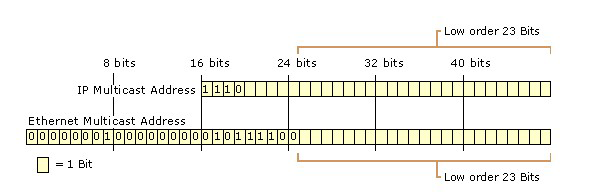
\includegraphics[width=0.8\linewidth]{fig/ip_mac.png}
	\end{figure}
	如224.0.1.5写为16进制是0xE0-00-01-05,取低23位,得到MAC完整地址为0x01-00-5E-00-01-05
\end{itemize}

地址解析协议(address resolution protocol, ARP)可以\underline{将IP地址映射为MAC地址}\footnote{也有将也有MAC映射为IP地址的协议}
\begin{itemize}
	\item ARP请求广播帧(谁的IP地址是XXX),ARP响应单播帧(返回MAC地址),IP地址与MAC地址的端口号相同
	\item 没有超时重传机制,超时没有收到响应则丢弃引发ARP查询的IP分组
	\item 源主机获得的映射结果缓存在ARP表中,TTL一般为2到20分钟
	\[\lrang{\text{IP address},\text{MAC address},\text{TTL}}\]
	\item 当收到ARP请求,目的主机会\textemph{缓存}源主机的映射,其他主机如果已缓存该映射,则会\textemph{重置TTL}
	\item 也可直接将映射加入ARP缓存,称为静态ARP映射,不会因超时而删除
	\item 源硬件地址和协议地址、目标协议地址都知道,但\textemph{目的硬件地址}不知
\end{itemize}
\begin{figure}[H]
	\centering
	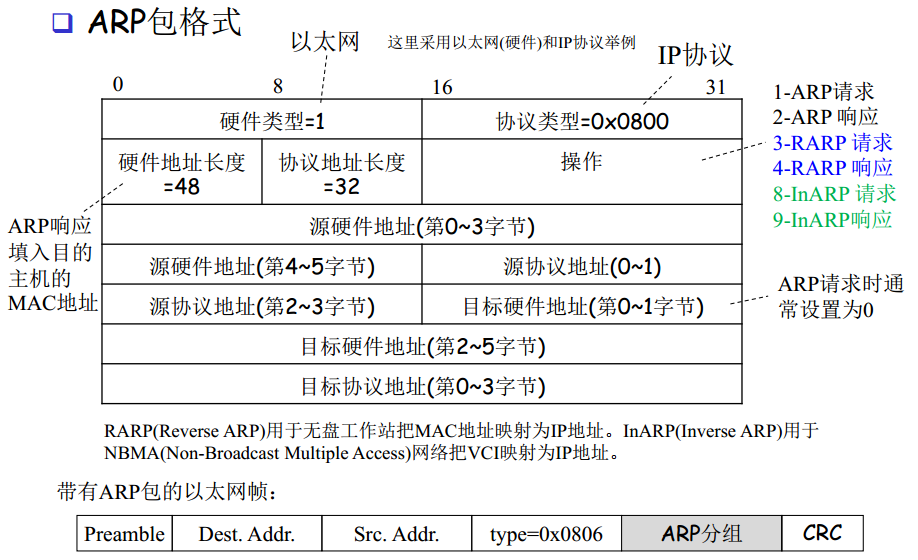
\includegraphics[width=0.7\linewidth]{fig/ARP.PNG}
\end{figure}

可以用ARP请求来确定一个IP地址在以太网中是否被使用,如果没有响应则说明没有使用。

\subsubsection{动态主机配置协议}
DHCP协议(Dynamic Host Configuration Protocol)用于主机在加入网络时\textemph{动态租用}IP地址,用UDP,四个步骤如下:
\begin{itemize}
	\item DHCP发现(discover)
	\item DHCP提供(offer): 还可以指出DHCP中转服务器,使多个网络可以共享一个DHCP服务器(通过DHCP discover的域名选项进行区分)
	\item DHCP请求(request):从多个响应的服务器中选择一个,并通告其它服务器已拒绝了它们的offer
	\item DHCP确认(ACK)
\end{itemize}

\subsubsection{因特网控制消息协议}
因特网控制消息协议(Internet Control Message Protocol, ICMP)用于主机或路由器发布网络级别的控制消息,主要是出错/丢包后将信息发回给源主机,如
\begin{itemize}
	\item 回响请求和答复消息(ping)(类型8):\underline{超时}是\textemph{回来的路找不到};而\underline{主机不可达}是\textemph{去的路找不到,中途原路返回}
	\item 不可达消息(类型3):用目的地址未查到匹配的路由项、需要分段但不可分段(DF=1)、网络/主机/协议/端口不可达,数据部分填原IP头部+原IP数据部分的头64b
	\item 源端抑制(类型4):控制源主机发送速度
	\item 重定位消息(类型5)
	\item 时间超时消息(类型11):TTL减到0、数据报重组超时
	\item 参数问题(类型12):坏的IP头部、缺少必要选项
\end{itemize}

\begin{example}
	主机和路由器通过三个以太网连接:[H1]-N1-[R1]-N2-[R2]-N3-[H2]。主机和路由器的每个接口的IP地址都配置正确。如果除了一种配置其他配置都是正确的,问导致以下问题的原因,并给出ping返回的结果?
	可选项:
	\begin{itemize}
		\item [A.]R1没有配置N3的静态路由指向R2
		\item [B.]R2没有配置N1的静态路由指向R1
		\item [C.]H1没有配置默认路由指向R1
		\item [D.]H2没有配置默认路由指向R2
	\end{itemize}
\end{example}
\begin{analysis}
	连上网后邻近的路由表端口就会被自动添加入本机的路由表,而且处于“在链路上”/直连的状态,故在路由表中查到R1左侧端口的路由表项,发现是直连网,会直接封装成帧发送出去,到达后路由器通过同样的物理网络发送ICMP包回来,故H1 ping R1左侧端口必然可以ping通(除非本机的IP协议出现故障)。
	\begin{enumerate}
	\item H1可以ping通R1左边接口的IP地址但是ping不通R1右边接口的IP地址:\underline{C,ping返回主机不可达}。
	由于H1没有配置默认路由,故ping R1右侧端口将直接在本机路由表项中找不到,进而丢弃,在主机出口处就直接返回不可达消息。
	\item H1可以ping通R1右边接口的IP地址但是ping不通R2左边接口的IP地址:\underline{B,ping返回超时}。
	ping通R1右侧接口说明H1配了默认路由,ping R1右侧接口时匹配上默认路由,故转发给R1,R1又通过查路由表项,发现是自己右端端口,直连网到达,然后返回ICMP包。
	正常来讲,在R1路由表项中会有后续网络的路由表项,ping R2左侧时匹配上并发送给R2。
	但由于R2没有配置N1的静态路由,导致ICMP数据报无法返回,在R2路由表中查不到对应路由表项,进而被丢弃,因为没有返回H1,故是超时。
	\item H1可以ping通R2左边接口的IP地址但是ping不通R2右边接口的IP地址:\underline{A,ping返回主机不可达}。与(1)类似的道理。
	\item H1可以ping通R2右边接口的IP地址但是ping不通H2的IP地址:\underline{D,ping返回超时}。与(2)类似的道理
	\end{enumerate}
\end{analysis}

\begin{example}
	ping可以在子网中产生一个广播帧,请给出并解释方法。
\end{example}
\begin{analysis}
	ping本网一个不存在的IP地址,因为ARP映射表中肯定没有,所以会发送ARP请求。ARP请求就是广播帧。或者直接ping对本网的广播,例如:ping 192.168.1.255,这个ICMP消息会用广播帧封装。
\end{analysis}
% http://www.linkwan.com/gb/tech/htm/908.htm

% \begin{example}
% 	一台路由器连接两个子网(以太网): N1-[R1]-N2。如果一台主机从一个子网移到另一个子网,并修改为另一个子网的IP地址,如何增加路由器的功能使这台主机还可以接收到用原IP地址发给它的数据报?
% \end{example}
% \begin{analysis}
% 	利用ARP协议,当其它主机在N1查询该主机的原IP地址的MAC地址时,R1要用自己的MAC地址进行响应。其它主机就会把IP数据报用帧发给R1,R1再转给该主机(位于N2中)。具体可查ARP代理
% \end{analysis}
% \begin{example}
% 	用一个交换机连接主机H1和H2。H1如何可以窃听到本网络中任何发给H2的IP数据报?
% \end{example}
% \begin{analysis}
% 	对任何用H2的IP地址查询H2的MAC地址的ARP请求,H1都要尽快用自己的MAC地址发出ARP响应。H1也可以用H2的IP地址和自己的MAC地址进行主动查询。
%% 交换机端口镜像Port Mirroring, also known as SPAN (Switched Port Analyzer) 实现监听
% \end{analysis}
% \begin{example}
% 	如果一个路由器连接了两个以太网,如何采用DHCP协议让这两个以太网可以共用一个DHCP服务器?
% \end{example}
% \begin{analysis}
% 	这里假设DHCP服务器只能接入其中一个子网,并具有两个子网的地址池可分配,路由器作为DHCP中继代理:
% 	当另一个子网的DHCP客户机广播请求地址租赁时,中继代理服务器就会把这个消息转发给另一子网中的DHCP 服务器,然后再将DHCP服务器返回的分配IP地址的消息转发给DHCP客户机,从而协助DHCP客户机完成地址租赁。
% 	DHCP服务器要根据DHCP中继代理给出的子网信息确定分配给客户机哪个子网的地址。
%% DHCP Relay(中继) 多个局域网共享一个DHCP服务器 https://www.netmanias.com/en/post/blog/6004/dhcp-network-protocol/what-is-a-dhcp-relay-agent
% \end{analysis}
% \begin{example}
% 	当一台主机要向远方的另一台主机发送很多数据报。如果它希望这些数据报中途不要分段以节约路由器的时间,这就要找到路径上最小的MTU,有何方法?假设这段时间该路径不会改变。
% \end{example}
% \begin{analysis}
% 	将数据报中的DF置为1,则路径上所有小于该包的MTU都会被丢弃,然后传递回一个类型3代码4的ICMP包(需要分段但不可分段),进而使得源主机减少它的路径MTU。最终直到MTU足够小以至于走完整条路径都不需要分段,此时获得的MTU就是路径最小MTU。
%% Path MTU Discovery 用于寻找路径上最小MTU

% 	Ping远端主机,每个数据报的DF均设置为1(即不允许分段),ICMP有效载荷的字节数从大到小变化,直到得到响应。也可以直接发送数据报而不用ping。
% \end{analysis}
% \begin{example}
% 	一台主机往远方的另一台主机发送数据报。如何可以通过数据报的TTL字段和ICMP协议依次(由近至远)得到整条路径上的路由器的IP地址(每个路由器只需要得到一个IP地址)? 假设这段时间该路径不会改变。
% \end{example}
% \begin{analysis}
% 	每一次发送一个数据报含有TTL,且TTL的值由1开始每次递增。路由器收到数据包后会将TTL减1,然后丢弃那些已经减到0的数据报,并返回ICMP超时包,进而可以获得距离为1的那些路由器IP地址。如此往复直到数据报能够到达另一台主机,此时整条路径上的路由器IP地址就都得到了,这有点像广度优先搜索(BFS)的原理。

% 	不断ping另一台主机,并且TTL从1开始不断增加。查traceroute命令。
%% Traceroute 用于获得整条路径上的路由器IP地址
% \end{analysis}

\subsection{路由协议}
\subsubsection{有类网的路由选择算法}
利用数据包中的\textemph{目的地址}得到\textemph{目的网络号},然后查询\textemph{路由表}(routing table)/转发表(forwarding table)
\begin{itemize}
	\item 如果查询的结果为\textemph{直连网},则\textemph{下一跳(next hop)为空},直接把数据包从查出的接口转发到目的主机
	\item 否则,如果查询得到\textemph{下一跳}(路由器),则把数据包转发给下一跳
	\item 如果没有查到任何匹配项,则把数据包转发给\textemph{默认路由器}(也算查到)
	\item 如果没有设置默认路由,则\textemph{丢弃}该数据包
\end{itemize}

\subsubsection{无类网的路由选择算法}
无类网的路由表里有子网掩码
\begin{itemize}
	\item 匹配方法: 目的IP地址 \& 子网掩码 $==$ 子网号
	\item 最长匹配原则(The longest match rule): 当有多条路由都匹配时选择子网掩码最长(1的长度)的路由,因为更详细
	\item 从IP数据报中获取目的地址,利用目的地址\textemph{查路由表}(同有类网)
	\begin{itemize}
		\item 没有匹配项:\textemph{丢弃}该分组
		\item 有匹配项,下一跳接口为以太网:从\textemph{路由表中查出下一跳}的IP地址,通过\textemph{ARP协议}获得\textemph{目的MAC地址},\textemph{封装成帧}发送,要遵守\textemph{以太网协议(CSMA/CD)}
		\item 有匹配项,没有下一跳,匹配项接口为以太网:直接取\textemph{IP数据报中的目的IP地址}(已经到达了)或用IP分组的目的地址查询MAC地址,封装成帧发送
		\item 有匹配项,下一跳接口为直连网(PPP)(或没有下一跳,匹配项接口为PPP):将数据报直接\textemph{封装成帧}发送,不需要目的地址(放到物理网络中自然会到达)
	\end{itemize}
	\item 每到一个路由器都将帧拆出来,再重新封装,目的和源MAC地址(上一跳路由器MAC地址)全要发生变化
\end{itemize}
注意:路由表中每一行的\textemph{下一跳和接口必然处于同一物理网络中}

\begin{example}
	给定目的地址求下一跳
\begin{figure}[H]
	\centering
	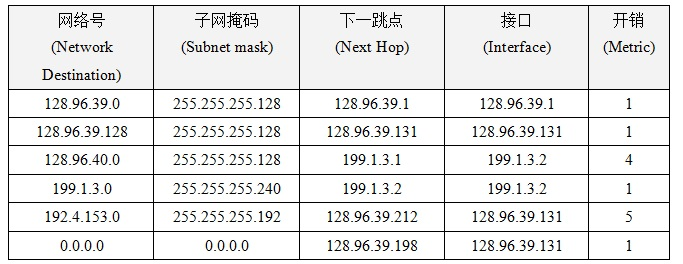
\includegraphics[width=0.8\linewidth]{fig/router_table_example.jpg}
\end{figure}
\end{example}
\begin{analysis}
	结果如下
	\begin{center}
		\begin{tabular}{cc}\hline
			目的地址 & 下一跳\\\hline
			192.4.153.17 & 128.96.39.212\\
			128.96.39.10 & 128.96.39.1\\
			128.96.40.12 & 199.1.3.1\\
			128.96.40.151 & 128.96.39.198\\
			192.4.153.90 & 128.96.39.198\\\hline
		\end{tabular}
	\end{center}
\end{analysis}

\begin{example}
	实战分析:“在链路上”意味着是\textemph{直连网},“网关”相当于\textemph{下一跳},“接口”直接\textemph{用IP地址标注}
	\begin{figure}[H]
		\centering
		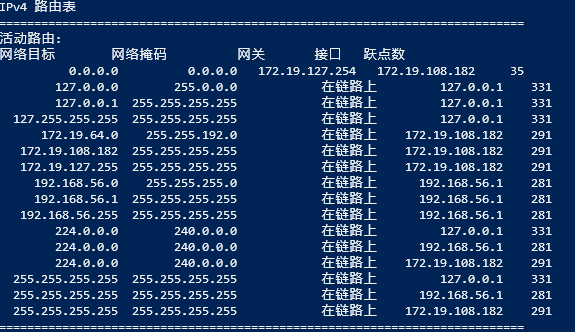
\includegraphics[width=0.6\linewidth]{fig/my-router-table.png}
	\end{figure}
\end{example}
\begin{analysis}
	网卡接上网络后,将会自动添加路由表项(直连网),一般也会将默认网关设好,即下一跳指向最近的路由器。
	\begin{enumerate}
		\item 0.0.0.0/0:默认路由,即其他项匹配不上的都会被送至172.19.108.182的接口,\\然后发送到172.19.127.254(默认网关,校园网私有地址,这是WiFi协议)
		\item 127.0.0.0/8:环回网络,发给自己
		\item 127.0.0.1/32:环回网络,本地地址(内部地址,其他是外部地址都需要经过网络层防火墙)
		\item 172.19.64.0/18:校园网内部网络,通过默认网关发出
		\item 192.168.56.1/32:VirtualBox虚拟机网卡接口IP
		\item 224.0.0.0/4:从跃点数较小(281)的端口192.168.56.1发出去,在无线网络中多播(接口不一样,因此要在路由器里写两项,一项内部一项外部)
		\item 255.255.255.255/32:在无线网络中广播
	\end{enumerate}
\end{analysis}
% 点到点可以路由器端口不用配IP地址,但以太网一定要配,因为可能有交换机
% https://blog.csdn.net/xiaohuima_dong/article/details/47777989
% https://www.rootusers.com/how-to-display-routing-table-in-linux/

\begin{example}[综合题]
	在下图中,R1和R2为路由器,S1为二层交换机,S2为三层交换机并配置了VLAN10和VLAN20的虚接口。R1到R2为一个配置了IP地址并使用PPP协议的点到点网络,其它四个(VLAN10,VLAN20,R1-R10,R2-H5)子网都是以太网。如果所有主机、三层交换机和路由器都正确配置了接口的IP地址,三层交换机和路由器都启动了OSPF协议,R1的默认路由指向R10并被发布到OSPF协议,问:H1 ping H3、H1 ping H4、H1 ping H5时依次经过了哪些设备(主机和路由器)以及它们分别使用了以下哪种协议?
	\begin{figure}[H]
		\centering
		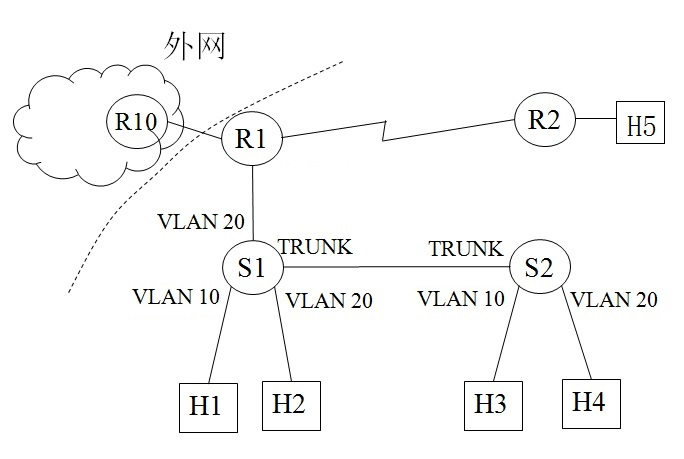
\includegraphics[width=0.6\linewidth]{fig/route_all_example.jpg}
	\end{figure}
	可选项:
	\begin{enumerate}
\item 透明网桥算法(带VLAN)
\item 802.1Q协议(trunk)
\item 以太网协议
\item ARP协议(IP地址为下一跳)
\item ARP协议(IP地址为IP分组的目的地址)
\item 查询路由表
\item PPP协议
\item 从收到的帧中取出IP分组
\item 网络层从上层收到数据并封装为IP分组
\item [A.] 匹配了默认路由
\item [B.] NAT
	\end{enumerate}
\end{example}
\begin{analysis}
	\begin{itemize}
		\item H1 ping H3 $\to$ H1:9653  S1:123   S2:13  H3:8
		\item H1 ping H4 $\to$ H1:9643  S1:123   S2:8653 H4:8
		\item H1 ping H5 $\to$ H1:9643  S1:3123   S2:3286423 S1:3213 R1:867 R2:8653 H5:8
		\item H1 ping 外网 $\to$ H1:9643  S1:3123   S2:3286A423 S1:3213 R1:86AB43 R10:386A...
	\end{itemize}
\end{analysis}

\subsubsection{路由表的建立}
路由表可以由管理员手工建立,也可以由路由/路由选择协议(routing protocols)自动建立,建路由表是即记\textemph{最短路径}的下一跳。

路由协议即自动建立路由表,包括网络号、子网号、下一跳、接口、开销等。
所建立的路由分别称为\textemph{静态路由}和\textemph{动态路由}。
默认路由和直连路由都是静态路由。

整个因特网实际上由很多机构进行管理。每个机构管理自己的网络,它们有权决定采用什么协议和网络控制策略。这样在\textemph{同一个机构}管理下的\textemph{网络}称为一个\textemph{自治系统}(autonomous systems, AS)。因特网实际上是由很多自治系统构成的。
\begin{itemize}
	\item 用于在AS\textemph{内部}(Intra-AS)建立动态路由的路由协议称为\textemph{内部网关协议}(Interior Gateway Protocols, IGP)。例如,\underline{RIP协议}和\underline{OSPF协议}。一个AS通常运行单一IGP。
	\item 用于在AS\textemph{之间}(Inter-AS)建立动态路由的路由协议称为\textemph{外部网关协议}(Exterior Gateway Protocol, EGP)。例如,\underline{BGP协议}。
	\item 运行同一个IGP协议的连通区域也称为路由选择域(routing domain)。一个AS可以运行多个IGP协议,形成多个路由选择域。
\end{itemize}

路由算法(Routing algorithm):路由协议里用的算法, 由于两个路由器之间都有开销,可以建立一个图,找最短路径
\begin{itemize}
	\item 距离向量(distance vector, DV):BellmanFord $\to$ RIP
	\item 链路状态(link state, LS):Dijstra $\to$ OSPF
\end{itemize}

\subsection{内部网关协议}
\subsubsection{RIP协议}
路由信息协议(Route Information Protocol, RIP):\textemph{距离向量}算法的路由协议(问路),工作原理是\underline{采用邻居的路由表构造自己的路由表}。
\begin{itemize}
	\item 每\textemph{30秒}\footnote{太频繁会占用带宽}RIP路由器把它的整个路由表发送给邻居。具体实现时每个邻居会错开发送,30秒的时间也会随机变化一点。
	\item 初始时每个RIP路由器只有到直连网的路由,它们的距离为1。
	\item 到目的网络的距离以跳为单位。最大距离为15。距离16表示无穷大,即目的网络不可达。
\end{itemize}

具体算法:
当收到邻居发来的路由表(update packet),路由器将更新它的路由表
\[\lrang{\text{目的网络},\text{开销},\text{下一跳}}\]
\begin{enumerate}
	\item 收到路由的距离全部加1(即一跳的距离)
	\item 利用上述路由修改路由表:
	\begin{itemize}
		\item 把路由表中不存在的路由加入路由表
		\item 如果比路由表中的路由的距离更小,则更新该路由的距离为新距离,把下一跳改为邻居
		\item 如果路由已经存在且下一跳就是邻居,则必须进行更新
	\end{itemize}
	\item 如果路由存在,就要重置失效定时器
\end{enumerate}
RIP路由表的每一项都有TTL(Time-To-Live),用失效定时器(invalid timer)计时,超时则让该路由失效

\begin{example}
	路由器A-G运行RIP协议,每跳的距离为1。B和C是邻居。如果B和C此时的路由表如下所示:
\begin{center}
\begin{tabular}{ccc|ccc}\hline
路由器B目的网络 & 距离 & 下一跳 & 路由器C目的网络 & 距离 & 下一跳\\\hline
N1 & 5 & A & N1 & 3 & F\\
N3 & 3 & C & N3 & 6 & F\\
N6 & 2 & E & N6 & 3 & B\\
N9 & 5 & D & N7 & 3 & G\\
N10 & 1 & - & N9 & 5 & G\\
& & & N10 & 2 & B\\\hline
\end{tabular}
\end{center}
当路由器B接收到来自C的路由表之后对路由表进行自己的更新, 请写出更新之后B的路由表
\end{example}
\begin{analysis}
路由器B路由表更新后的结果为
\begin{center}
\begin{tabular}{ccc}\hline
目的网络 & 距离 & 下一跳\\\hline
N1 & 4 & C\\
N3 & 7 & C\\
N6 & 2 & E\\
N7 & 4 & C\\
N9 & 5 & D\\
N10 & 1 & -\\\hline
\end{tabular}
\end{center}
记得要更新下一跳的内容
\end{analysis}

\myhline
RIP协议存在的问题
\begin{itemize}
	\item 慢收敛:最短时间接近$0$(这样看更新时刻),最长时间$30(m-1)$,平均时间$15(m-1)$
	\item 计数到无穷:N1--R1--N2--R2--N3。在R1因N1失效而把N1的路由的距离改为16(无穷大)之后,R2将路由表发给R1
\end{itemize}

解决方案
\begin{itemize}
	\item 水平分割(split horizon)技术:从一个接口学来的路由不会从该接口发回去;依然会计数到无穷,三角形R1断了,R1先发,R2后发
	\item 毒性反转(poison reverse)技术:当一条路由变为无效之后,路由器并不立即将它从路由表中删除,而是将其距离改为用16后广播给邻居,使邻居所拥有的该路由立即失效,而不是等待TTL到期后删除,以迅速消除路由环路,这种方法称为毒性反转,距离为16的路由称为毒化路由(poisoned route)
	\item 抑制技术(hold down):距离被改为无穷大的路由在一段短时间(180秒)内其距离不允许被修改
	\item 触发更新(triggered update):一旦出现路由变化将立即把变化的路由发送给邻居。原有的30秒发一次完整的路由表依然不变(因触发更新可能丢失;路由表也可能出错;要用TTL清除无效路由)
\end{itemize}

\myhline
RIP协议的定时器
\begin{itemize}
\item 更新定时器(Update Timer)控制一个路由器如何定期把路由表发送给邻居。默认时间为30秒。
\item 一条路由的失效定时器(Invalid Timer)到期时被标记为无效路由(距离改为16)。路由被更新时其失效定时器会被重置。默认值为180秒。
\item 一条路由的清除定时器(Flush Timer)到期时该路由将从路由表中删除。路由被更新时其清除定时器会被重置。默认值为240秒。
\item 抑制定时器(Hold-down Timer)在路由的距离变为无穷大(包括收到毒化路由)时启动。在其到期之前不允许修改该路由的距离。默认值为180秒。
\end{itemize}
\begin{figure}[H]
	\centering
	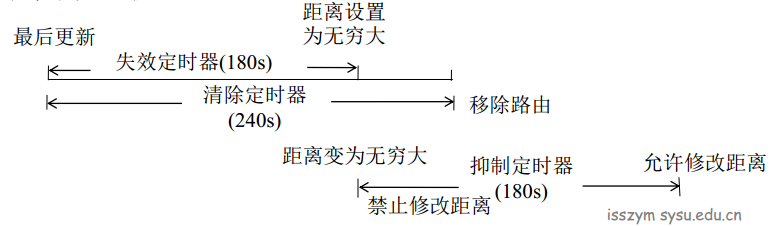
\includegraphics[width=0.7\linewidth]{fig/rip_timer.png}
\end{figure}

\myhline
RIP协议简单、容易实现。特点如下:
\begin{itemize}
\item 网络的直径不能超过16跳
\item 不允许把一个大网络分成多个区
\item 开销缺乏灵活性
\item 存在慢收敛问题和计数到无穷问题
\item 每30秒发送完整路由表会消耗大量的带宽
\item 实际运行的RIP协议具有如下特性:
\begin{itemize}
\item 可以保存多达6个等距离的路由在路由表中,默认为4个
\item 直连网的管理距离为0,RIP协议的距离为1
\end{itemize}
\end{itemize}

\subsubsection{OSPF协议}
开放最短路径优先协议(Open Shortest Path First, OSPF)采用\textemph{链路状态}路由算法,可能是在大型企业中使用最广泛的内部网关协议。
\begin{itemize}
\item 周期性地收集链路状态,并\textemph{扩散}给AS中的所有路由器
\item 用收到的链路状态建立整个AS的拓扑结构图
\item 利用Dijkstra算法计算到AS中所有网络的最短路径
\item 利用这些路径上的下一跳建立路由表
\end{itemize}

\myhline
OSPF第一步需要将整个网络(AS)转化为AS的拓扑结构图。
\begin{itemize}
	\item 每一个路由器和每一个网段(多路访问网络/\textemph{点到点网络})都作为一个结点
	\item 每个\textemph{中转网}(transit network),要选举一个直连路由器作为其指定路由器(designated router, DR)
	\item 中转网只有入边有权,出边都没有
	\item 如果点到点网络没有配置IP地址,则该结点可去除
	\item \textemph{末端网}(stub network)即不再连其他路由器的网络,管理员设的
	\item 每一个\textemph{路由/网段}都有自己的链路状态通告(Link State Advertisement, LSA)(2种LSA)
\end{itemize}
\begin{example}
	如下图,有3个router LSA,而只有1个network LSA(环回网络是末端网)
\begin{figure}[H]
	\centering
	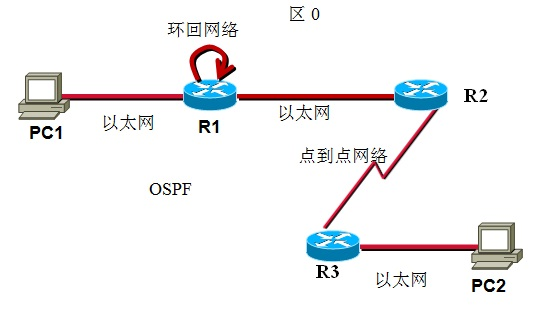
\includegraphics[width=0.45\linewidth]{fig/ospf_lsa.jpg}
\end{figure}
\end{example}

详细过程如下
\begin{itemize}
	\item 发现邻居:每10秒向邻居发送Hello分组,如果40s(dead interval)都收不到邻居发来的Hello分组,则把到邻居的链路标记为失效。多路访问网络采用多播(224.0.0.5, all OSPF routers)发送Hello分组。一个Hello分组包含优先权、已知的邻居(收到过Hello)、DR和BDR
	\item 完全相邻:在发现邻居之后, OSPF路由器将与邻居交换链路状态数据库中的LSA,请求得到更新的或者没有的LSA。在与邻居的链路状态数据库变得完全一样时,它们就处于完全相邻状态(fully adjacency)
	\item 生成LSA:每\textemph{30分钟}或链路变化时,每个OSPF路由器会生成router LSA,中转网的DR会生成network LSA
	\item 扩散LSA:产生的LSA立即封装为Update分组,被可靠地扩散出去 (需要确认)。每次产生的LSA的序号会加1。序列号越大表示越新。若通过收到多个LSA,由发出此LSA的路由器ID(发通告路由器),链路状态和序列号唯一确定。通过序号,也可以防止扩散形成回路,第二次收到来自相同的发通告路由器、相同LSA类型和相同序号的LSA将丢弃它
	\item 收集LSA:路由器收集到LSA之后,用新LSA替换链路状态数据库中旧LSA。如果一个LSA在60分钟(max age)没有被更新,它将从链路状态数据库移除
	\item 计算最短路径:当链路状态数据库被改变时, OSPF路由器将利用Dijkstra算法计算到所有网络的最短路径。
	\item 建立路由表:利用得到的最短路径产生路由表
\end{itemize}
\begin{example}
	写出对应的网络和路由LSA
	\begin{figure}[H]
		\centering
		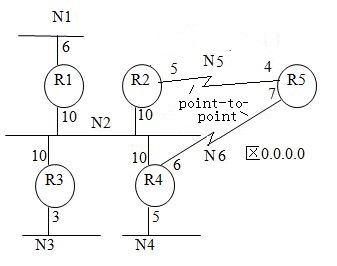
\includegraphics[width=0.4\linewidth]{fig/ospf_example.jpg}
	\end{figure}
\end{example}
\begin{analysis}
	举例如下,中转网LSA到其他路由开销为0!
	\begin{center}
	\begin{tabular}{ccc|ccc|cc}\hline
		R1 LSA & 开销 & 链路类型 & R2 LSA & 开销 & 链路类型 & N2 LSA & 开销\\\hline
		N1 & 6 & 末端网 & R5 & 5 & 点到点 & R1 & \textemph{0}\\
		N2 & 10 & 中转网 & N5 & 5 & \textemph{末端网} & R2 & 0\\
		& & & N2 & 10 & 中转网 & R3 & 0\\
		& & & & & & R4 & 0\\\hline
	\end{tabular}
	\end{center}
	R5的路由表,中转网只算一次开销!
	\begin{center}
	\begin{tabular}{ccc|ccc}\hline
		目的 & 开销 & 下一跳 & 目的 & 开销 & 下一跳\\\hline
		N1 & 20 & R2 & N4 & 12 & R4\\
		N2 & 14 & R2 & N5 & 4 & -\\
		N3 & 17 & R2 & N6 & 7 & -\\\hline
	\end{tabular}
	\end{center}
\end{analysis}

\myhline
OSPF协议采用路由器ID(RID)标识每一个路由器。
路由器ID由以下方法得到:
\begin{itemize}
	\item 使用直接配置的RID
	\item 所有活动环回接口中最大的IP地址
	\item 所有活动物理接口中最大的IP地址
\end{itemize}
除非路由器重启、所选接口故障或关闭或IP地址改变、重新执行了router-id命令,RID都将保持不变。

% 透明网桥来了就转,数据报中没有标识
% 但对于OSPF来说,有序号,知道收到过一次,就把它丢了,管理数据所以可以这样弄

\myhline
指定路由器的选举方法:
\begin{itemize}
	\item 当多路访问网络重启时,选择DR的过程就开始了。在等待时间结束(Wait Time/Dead Interval, 40s)时,带有\textemph{最高和次高优先权}的路由器分别成为DR和BDR(Backup DR)。如果优先权相同,RID更大的成为DR,次大的成为BDR。
	\item 如果路由器不希望参与选举,则应该把优先权设置为0。如果优先权相同,具有\textemph{更高RID}的路由器成为DR。如果收到的Hello列出了DR(RID不是0.0.0.0),路由器成为DR。
	\item 如果一个新的路由器在选举之后到达或者有路由器修改为更高的优先权,它也不可能抢占现存的DR/BDR和变为DR/BDR。
	\item 当DR失效时, BDR成为DR,将开始一个新的选举过程来选出BDR。
	\item 一个多路访问网络中的OSPF路由器只与DR和BDR建立相邻关系。
	\item 收到一个LSA后,一个多路访问网络中的OSPF路由器将把它首先多播(224.0.0.6)给DR和BDR,然后 DR再把它多播(224.0.0.5)给所有OSPF路由器
\end{itemize}

\myhline
LSA具有多个定时器
\begin{itemize}
	\item 每10秒(Hello Interval)向邻居发送一次Hello,4倍的hello interval(Dead Interval,40s)没有收到邻居的Hello就认为邻居失效。
	\item 每30分钟会产生新的LSA,最小间隔时间为5s。
	\item 每个LSA都有年龄字段(age),发给邻居时被设置为0,在链路状态数据库中age会不断增长,增长到Max Age(默认为60分钟)时LSA被标记为失效。失效的LSA会被扩散到整个AS,令AS的所有路由器把该LSA从链路状态数据库中移除。
	\item 存储在链路状态数据库中的LSA每10分钟会被计算校验和,如果有错将被删除。
	\item 接收来自邻居的LSA的最小间隔时间为1s。
	\item 计算最短路径的最小间隔时间为10s。
\end{itemize}

\myhline
OSPF特点:
\begin{itemize}
	\item 所有的OSPF消息都要认证 (防止恶意入侵)。
	\item 路由表中允许多个\textemph{相同开销}的路经存在(RIP只允许一条路径),可以实现负载均衡。
	\item 对于每条链路,允许同时有多个(TOS)开销。
	\item 多播OSPF(MOSPF)使用与OSPF相同的链路状态数据库(思科路由器不支持)
	\item 在大型路由选择域中OSPF可以\textemph{分区}。
	\item 比RIP\textemph{收敛快而且更安静}。
	\item 实现起来更复杂,需要更多的\textemph{计算开销}。
\end{itemize}

\subsubsection{两种算法比较}
\begin{center}
\begin{tabular}{|c|c|c|}\hline
	& LS & DV\\\hline
消息复杂性 & n个节点, E条链路, 要发送$O(nE)$条消息 & 只在邻居之间交换消息\\\hline
收敛速度 &
\begin{tabular}{l}
$O(n^2)$算法需要$O(nE)$条消息\\
可能会震荡
\end{tabular} &
\begin{tabular}{l}
收敛时间变化\\
可能出现路由循环\\
计数到无穷问题
\end{tabular}\\\hline
健壮性\footnote{路由器失效时会出现什么情况?} &
\begin{tabular}{l}
可能通告不正确的链路开销\\
每个节点只计算自己的路由表
\end{tabular} &
\begin{tabular}{l}
DV节点可能通告不正确的路径开销\\
每个节点的路由表被其它节点所用\\
错误会通过网络传播开
\end{tabular}\\\hline
\end{tabular}
\end{center}


\subsection{外部网关协议}
\subsubsection{EGP协议}
外部网关协议(Exterior Gateway Protocol, EGP)既是分类也是协议,只能对树型,还要判回路

\subsubsection{BGP协议}
边界网关协议(Border Gateway Protocol, BGP)可以用于图,随便连
\begin{itemize}
\item 采用可靠扩散(reliable flooding)的方法把AS内的网络的信息传遍整个因特网
\item 每个AS需要分配一个号码。与IP地址分配相同,全局AS号(1 - 64511)由ICANN的下属机构进行统一分配。 64512 - 65535为私有AS号。
\end{itemize}

\myhline
工作原理
\begin{itemize}
\item 运行了BGP协议的路由器被称为BGP路由器,所运行的BGP协议称为BGP发言人(speaker),其他路由器为内部路由器
\item 在BGP路由器之间可以通过TCP连接(端口号为179)建立相邻关系,由AS管理员指定,也可以采用自动产生(重发布)和聚合产生。这些指定网络只有发布路由表中存在才会被改路由器扩散出去。如果它们失效,则会把撤销路由的消息扩散出去。
\item AS内的两个BGP路由器之间建立的相邻关系称为iBGP(interior BGP)相邻关系,而位于不同AS的两个BGP路由器之间建立的相邻关系称为eBGP(exterior BGP)相邻关系
\item  BGP协议所扩散的网络前缀/网络号称为网络层可达信息(Network Layer Reachablility Information, NLRI),BGP路由器可以把NLRI连同它们的属性一起通过相邻关系扩散给邻居,进而扩散到因特网中所有的BGP路由器
\item BGP路由器在NLRI引入BGP协议时扩散一次,并不定期扩散
\end{itemize}
\begin{figure}[H]
	\centering
	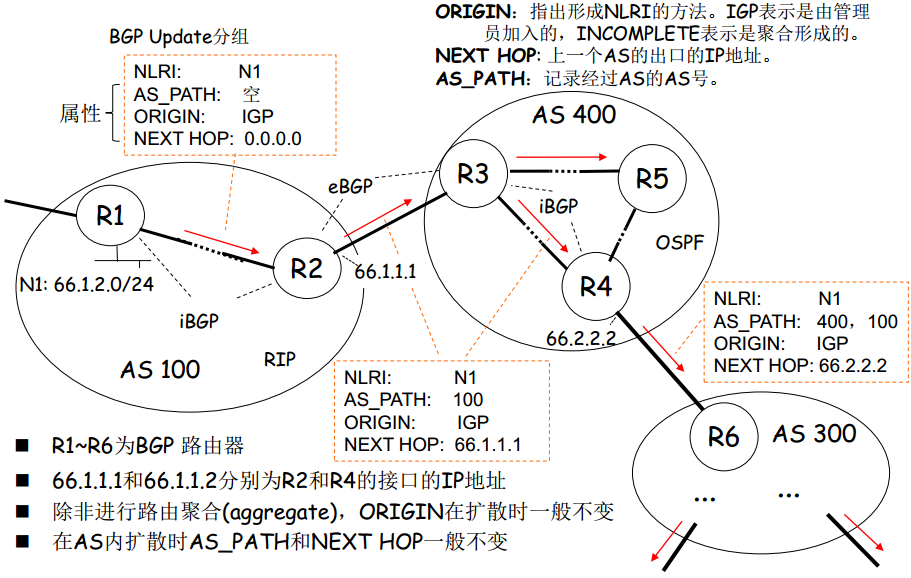
\includegraphics[width=0.8\linewidth]{fig/NLRI.png}
\end{figure}

\begin{itemize}
\item BGP路由器可以聚合若干NLRI网络形成一个新的NLRI。
\item 如果从多条路径收到同一个NLRI,在默认情况下选择AS-PATH中AS数最少的路径。
\item BGP路由器根据NLRI的属性NEXT HOP查询IGP路由表得到NEXT HOP, 就可以使用该路由。如果没有查询到匹配项,则丢弃该NLRI。
\item 如果设置了IGP同步并且NLRI在IGP路由表中没有匹配项,该NLRI不能转发给eBGP邻居。
\item BGP路由器可以把多个路由聚合(aggregate)为一个路由,其NLRI的ORIGIN属性要改为IMCOMPLETE。
\item 如果iBGP邻居之间的路由要经过内部路由器,那么就要给IGP路由表中注入AS外的路由,或者通过隧道技术连接iBGP邻居。
\item 内部路由用默认路由转到BGP路由,然后连到世界上任一台路由器;
在路径上的路由不可设默认路由,否则只能转到一个方向
\end{itemize}

内部路由如何发到外部
\begin{itemize}
\item 查next hop,BGP注入IGP路由,但非BGP路由承受不住;或将路径上所有路由都变为BGP路由
\item 在IP层运用了虚电路(等于挖了个隧道),不用记中间路由器,现在都用这种方式
\end{itemize}

\myhline
防止出现回路的方法:
\begin{itemize}
\item 内部:从iBGP邻居收到的NLRI Update分组不能再发给邻居
\item 之间:利用AS Path防止回路
\end{itemize}

\subsection{IP多播}
\subsubsection{概述}
访问同个网站,只发一次请求并回收;但单播访问同一个网站也要多次发送
\begin{itemize}
\item 单播:浪费带宽,增加CPU负担,扩展性差
\item 多播:可扩展(视频直播非常有优势)
\end{itemize}
\begin{figure}[H]
	\centering
	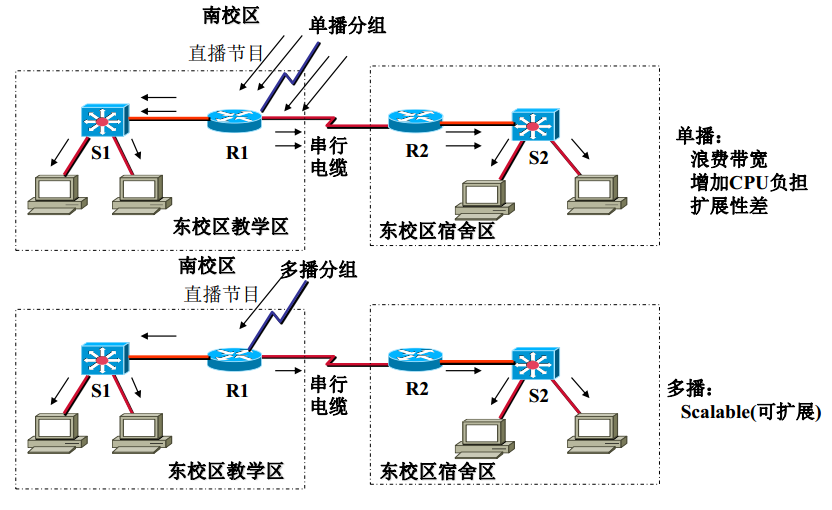
\includegraphics[width=0.8\linewidth]{fig/multicast.png}
\end{figure}

\subsubsection{多播IP地址}
\begin{center}
\begin{tabular}{|l|p{15em}|}\hline
多播地址范围 & 用法\\\hline
\textemph{224.0.0.0 - 239.255.255.255} & IPv4的多播地址空间\\\hline
224.0.0.0 - 224.0.0.255 & 由IANA分配的永久地址。路由器不转发目的地址为这些地址的IP数据包\\\hline
224.0.1.0 - 224.0.1.255 & 由IANA分配的永久地址。路由器会转发目的地址为这些地址的IP数据包\\\hline
232.0.0.0 - 232.255.255.255 & 用于指定源的多播应用\\\hline
233.0.0.0 - 233.255.255.255 & 由AS分配的全局多播地址\\\hline
239.0.0.0 - 239.255.255.255 & 私有多播地址\\\hline
其它地址 & 临时多播地址(transient address)\\\hline
\end{tabular}
\end{center}

\subsubsection{多种多播协议}
\begin{itemize}
\item 逆向路径广播:指定源的树\\
利用源地址查路由表,当一个路由器收到一个源地址为S发往组G的多播分组<S,G>时, 当且仅当该分组到来的接口在从该路由器到S的最短路径(Parent Link)上时,该路由器才在它的其它接口广播(flooding)该分组。(类DFS)
\begin{figure}[H]
	\centering
	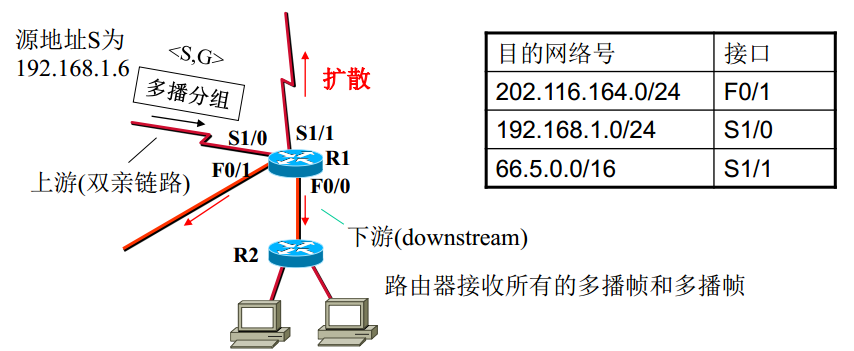
\includegraphics[width=0.8\linewidth]{fig/reverse_path_broadcasting.png}
\end{figure}
建路由表时源地址路径上一定是最短路径,每一次都往远的地方走,故一定没有回路
\item 逆向路径多播:对于每个多播地址G,每个源地址形成一棵树,即源特定组播树(source-specific multicast tree),然后剪枝\\
对于基于一个源地址的组播流,如果路由器的所有下游接口均无该组成员或已被剪枝,则它通过其双亲链路向上发送剪枝消息(Prune Message)。 路由器不会把多播分组从剪枝口转发出去\\
如果有新主机加入多播组,则要通过嫁接消息(Graft Message)逐级向上通知直到某个未被剪枝的
接口或者根路由器。\\
为了防止嫁接消息丢失引起转发受阻,路由器定期取消所有剪枝。
\end{itemize}

\myhline
\begin{itemize}
	\item 距离向量多播路由协议(Distanse	Vector Multicast Routing Protocol, DVMRP):在距离向量算法的基础上使用逆向路径多播算法实现的多播路由算法
	\item 协议无关多播-稠密模式(Protocol Independent Multicast - Dense Mode, PIM-DM)协议:逆向路径多播算法,路由器只需要知道到源主机的最短路径的接口,与使用什么内部网关协议无关
	\item MOSPF协议是另一种用于组成员稠密方式下的多播协议:如果使用OSPF协议,路由器可以通过Group Membership LSA把自己的哪些直连网有组成员的信息传遍整个AS,最后,所有AS的路由器都在原拓扑结构图上标志哪些(网络)节点有组成员。这样, 每个节点就可以计算出源节点到组成员的\textemph{最短路径多点播送生成树}。MOSPF路由器在收到多播分组时为每个源和多播组建造一颗生成树。由于计算量很大, MOSFP不适用于大型网络。Steiner树是总代价最小的分布树。 求Steiner树是NP问题。
	\begin{figure}[H]
		\centering
		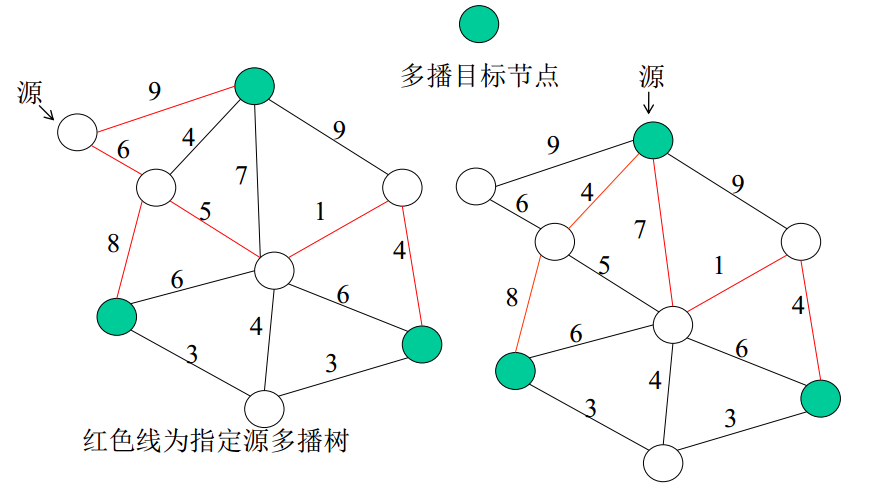
\includegraphics[width=0.6\linewidth]{fig/MOSPF.png}
	\end{figure}
	\item 协议无关多播-稀疏模式协议(Protocol Independent Multicast - Sparse Mode, PIM-SM)用实现于组成员稀疏情形下的多播
\end{itemize}

\myhline
因特网组管理协议(Internet Group Management Protocol, IGMP)用于路由器查询与它直连的网络上是否存在组成员
\begin{itemize}
	\item IGMPv1协议只能对某个接口查询所有组,如果三次查询在十秒内都没有收到响应报告,则认为该接口没有任何组成员。
	\item IGMPv2协议可以直接针对某个组进行查询,而且主机加入组和离开组都要发通告。
\end{itemize}